%\documentclass[10pt]{beamer}
%\documentclass[10pt,aspectratio=169]{beamer}
\documentclass[handout,10pt,aspectratio=169]{beamer}
%\includeonlyframes{current}
\usepackage{textcomp,colortbl}
\usepackage{amsmath, amssymb, etoolbox, bm, listings}
\usepackage{animate, multirow, hyperref, color, longtable}
\usepackage{makeidx, multicol}
\usepackage[retainorgcmds]{IEEEtrantools}
\hypersetup{
  colorlinks,
  urlcolor=blue
}

% These commands are from stack exchange. They are for creating the index of
% examples.
\makeindex
\newenvironment{theindex}
 {\let\item\par
  %definitions for subitem etc
  }{}
\newcommand\indexspace{}

\newcommand{\topic}{02}
\newcommand{\bb}{\mathbb}
\newcommand{\rlang}{\texttt{R} }
\newcommand{\ud}{\,\mathrm{d}}

%\includeonlyframes{current}
\setbeamertemplate{theorems}[numbered]
%\setbeameroption{show notes}
\undef{\example}
\theoremstyle{example}
\newtheorem{example}{\translate{Example}}

\DeclareMathOperator{\var}{var}
\DeclareMathOperator{\cov}{cov}
\DeclareMathOperator{\cor}{cor}
%\DeclareMathOperator{\dp}{dp}
\DeclareMathOperator{\ds}{ds}
\DeclareMathOperator{\dt}{dt}
\DeclareMathOperator{\du}{du}
\DeclareMathOperator{\dv}{dv}
\DeclareMathOperator{\dw}{dw}
\DeclareMathOperator{\dx}{dx}
\DeclareMathOperator{\dA}{dA}
\DeclareMathOperator{\dy}{dy}
\DeclareMathOperator{\dz}{dz}
\DeclareMathOperator{\dr}{dr}
\DeclareMathOperator{\dtheta}{d\theta}
\DeclareMathOperator{\SD}{SD}
\DeclareMathOperator{\Be}{Be}
\DeclareMathOperator{\Bin}{Bin}
\DeclareMathOperator{\Geom}{Geom}
\DeclareMathOperator{\Poi}{Poisson}
\DeclareMathOperator{\Exp}{Exp}

\DeclareMathOperator{\di}{d}
\newcommand{\ddx}{\frac{\di}{\dx}}
\newcommand{\ddz}{\frac{\di}{\dz}}
\newcommand{\ddxt}{\tfrac{\di}{\dx}}
\newcommand{\dydx}{\frac{\dy}{\dx}}
\newcommand{\dydxt}{\tfrac{\dy}{\dx}}
\newcommand{\pdx}[1]{\frac{\partial {#1}}{\partial x}}
\newcommand{\pdy}[1]{\frac{\partial {#1}}{\partial y}}
\newcommand{\rll}[1]{\texttt{#1}}

\usetheme{Boadilla}
\usecolortheme{dove}
%\usetheme[hideallsubsections]{PaloAlto}
% Control the style of bullets:
\setbeamertemplate{enumerate items}[circle]
\setbeamertemplate{section in toc}[circle]
\setbeamercolor{block title}{bg=cyan}
%setbeamercolor{block title}{bg=yellow}
\renewcommand<>\cellcolor[1]{\only#2{\beameroriginal\cellcolor{#1}}}

\setbeamertemplate{footline}[text line]{%
  \parbox{\linewidth}{\vspace*{-8pt}\insertshorttitle\hfill\insertshortauthor\hfill\insertpagenumber}
}
\setbeamertemplate{navigation symbols}{}

\title[]{ Containerisation with Docker}
\author[Topic \topic]{Vik Gopal}
\date{DSA3101 AY 22/23 Sem I}

%\usepackage{Sweave}
\begin{document}
\lstset{
  upquote=true,
  basicstyle=\ttfamily,
  backgroundcolor=\color{yellow!10},
  showstringspaces=false}
\maketitle
\section*{Outline}
\frame{\tableofcontents}

\section{Introduction to Docker}

\begin{frame}{What is Docker?}
\begin{itemize}
\item
  Docker is a platform for developing and sharing applications in
  \emph{containers}.
\item
  A container is a loosely isolated environment that contains all the
  packages needed to run an application.
\item
  Examples of applications are web servers, databases, and web
  applications such as dashboards.
  \begin{itemize}
  \item
    We are going to use it to develop custom web applications for
    serving a model, running a dashboard, or any other data science
    related front-end.
  \end{itemize}
\end{itemize}
\end{frame}

\begin{frame}{What is Docker?}
\framesubtitle{cont'd}
\begin{itemize}
\item
  Previously, we needed great technical know-how to install and
  configure related components on a single machine just for testing.
  (figure from book `Deploy ML Models to Production', Singh (2021))
\end{itemize}
\begin{center}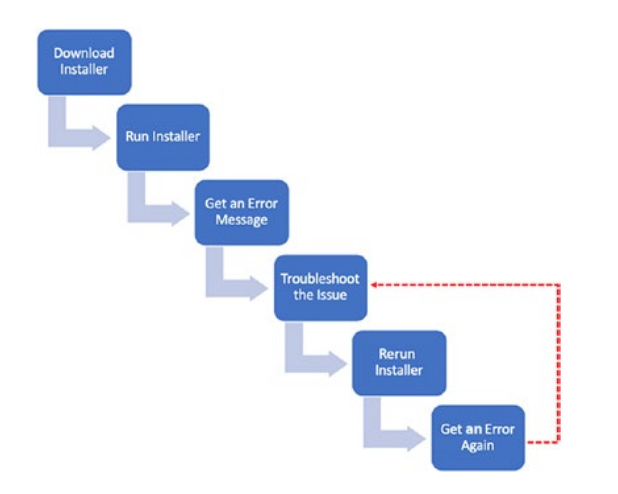
\includegraphics[width=0.5\linewidth]{figs/installation_without_docker} \end{center}
\end{frame}

\begin{frame}[plain]{Examples of Applications}
\begin{center}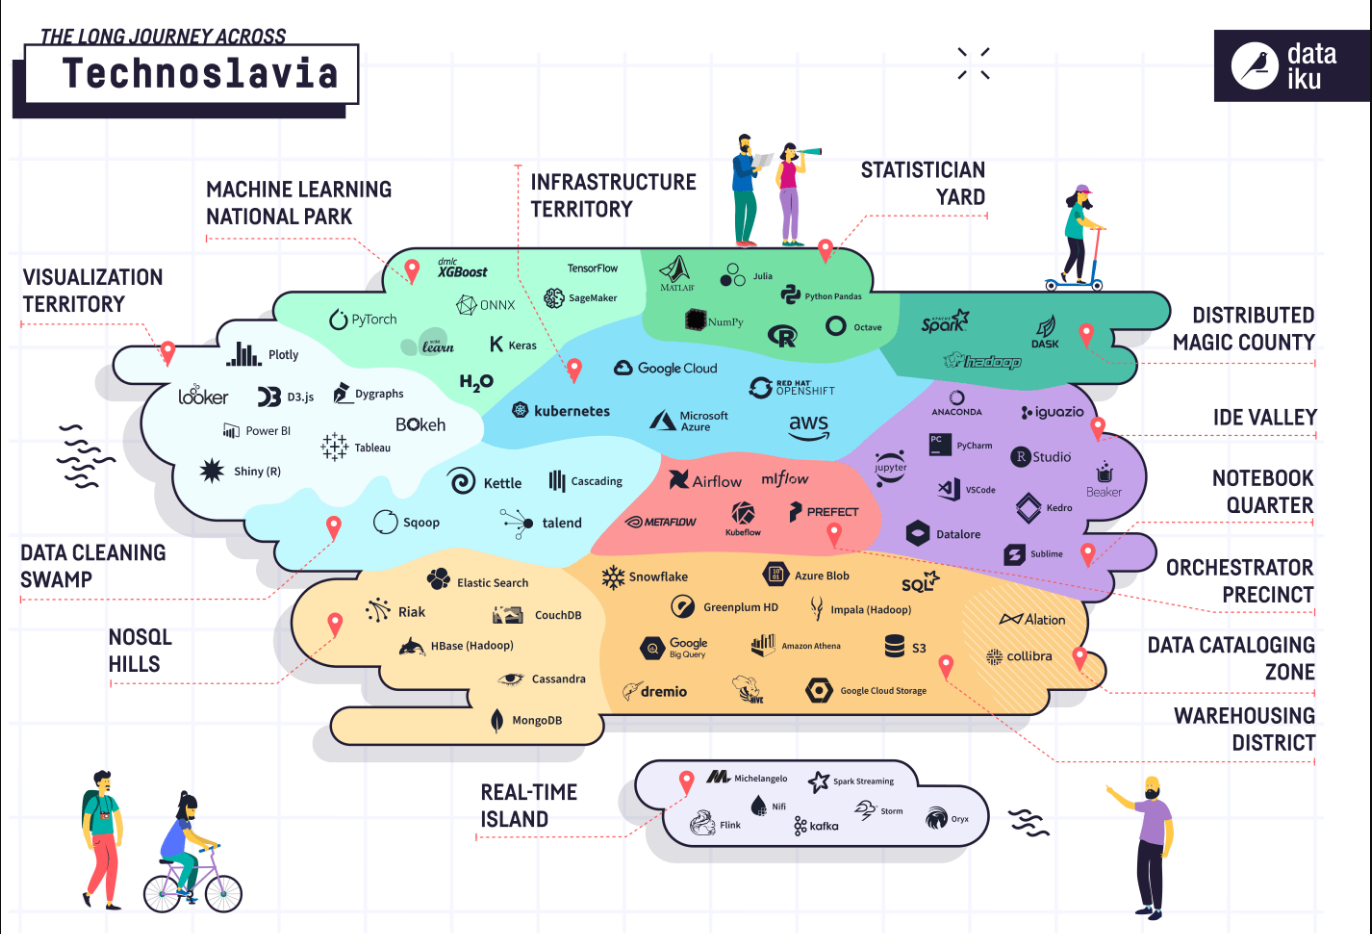
\includegraphics[width=0.6\linewidth]{figs/technoslavia} 
\end{center}
Figure from 
\href{https://blog.dataiku.com/technoslavia-the-fragmented-world-of-data-infrastructure-in-2021}{here}
\end{frame}

\begin{frame}[plain]{Examples of Applications}
\begin{center}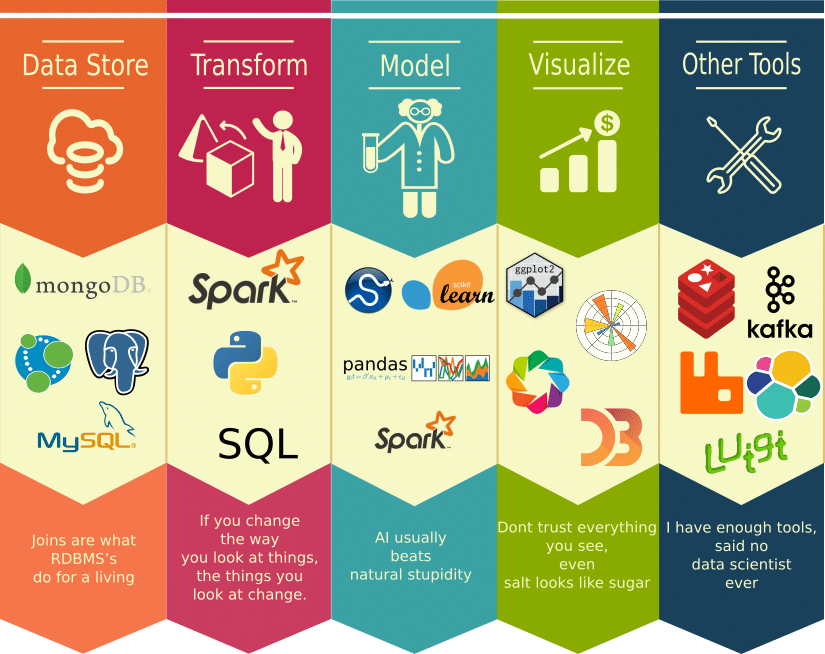
\includegraphics[width=0.55\linewidth]{figs/ds_stack_tools} \end{center}
Figure from
  \href{https://research.aimultiple.com/data-science-tools/}{here}.
\end{frame}

\begin{frame}{Why Learn About Containers?}
\begin{columns}[T]
\begin{column}{7.5cm}
\begin{block}{New skills needed}
    \begin{itemize}
    \item Need to integrate models with these tools.
    \item Need to demonstrate value with a PoC or MVP.
    \item Appreciate the data engineering pipeline better.
    \end{itemize}
\end{block}
\end{column}
\onslide<2->
\begin{column}{7.5cm}
\begin{block}{Benefits of containers}
\begin{itemize}
\item
  Continuous integration and delivery
\item
  Code developers can collaborate on containers. The same containers can
  be used for testing and production.
\item
  Containers can be developed in isolation before getting them to work
  with one another.
\item
  Fast, lightweight, scalable.
\end{itemize}
\end{block}
\end{column}
\end{columns}
\end{frame}

\begin{frame}{Containers vs. Virtual Machines}
  Before containers became popular, we would use virtual machines to run
  on a guest host machine. This required an entire OS, which hogged
  physical resources, on top of our own OS.
\begin{center}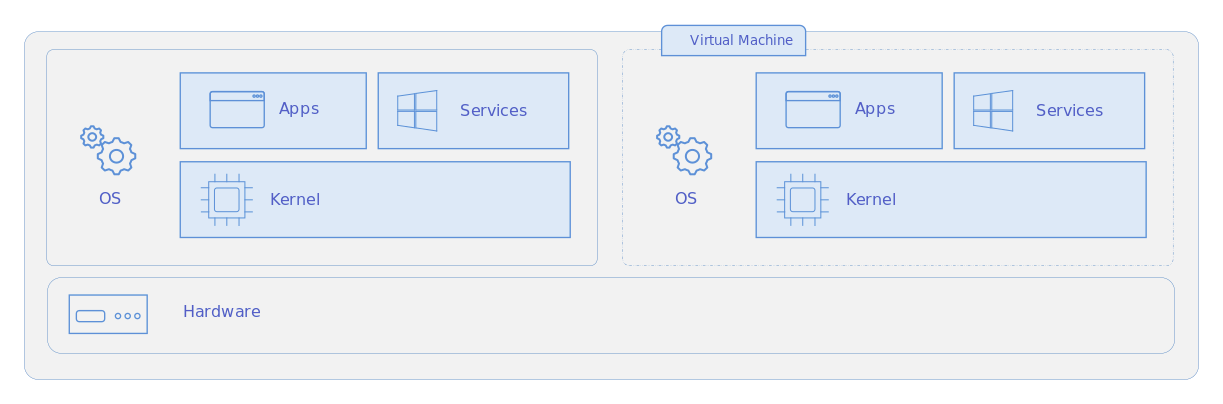
\includegraphics[width=0.75\linewidth]{figs/virtual-machine-diagram} \end{center}
\end{frame}

\begin{frame}{Containers vs. Virtual Machines}
\framesubtitle{cont'd}
  With containers, we can rely on the kernel of the host OS.
\begin{center}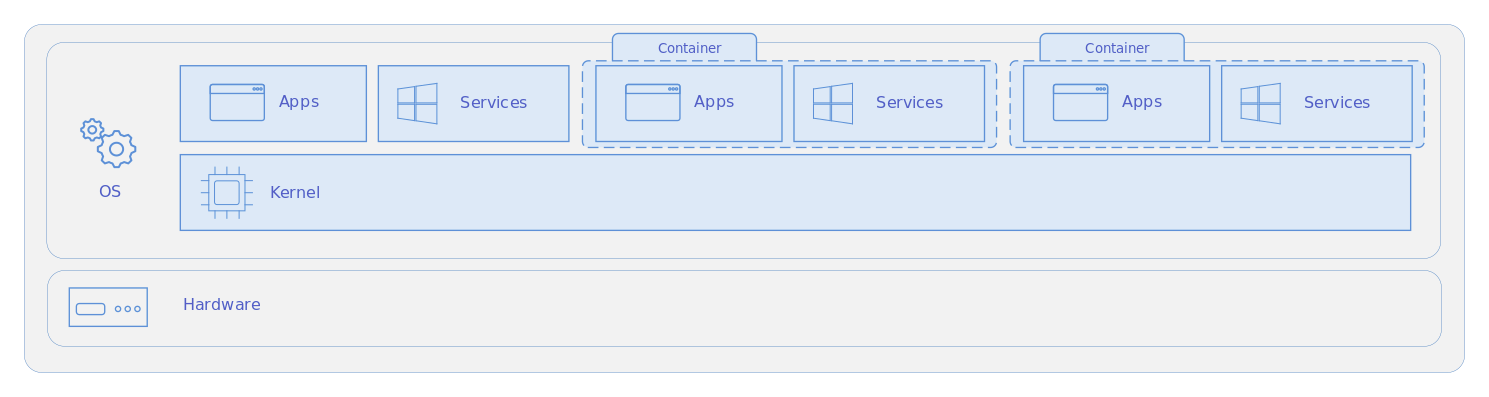
\includegraphics[width=0.75\linewidth]{figs/container-diagram} \end{center}
  Both figures from
  \href{https://docs.microsoft.com/en-us/virtualization/windowscontainers/about/containers-vs-vm}{Microsoft
  documentation on containerisation}.
\end{frame}


\begin{frame}[plain]{How Docker Works}

\begin{center}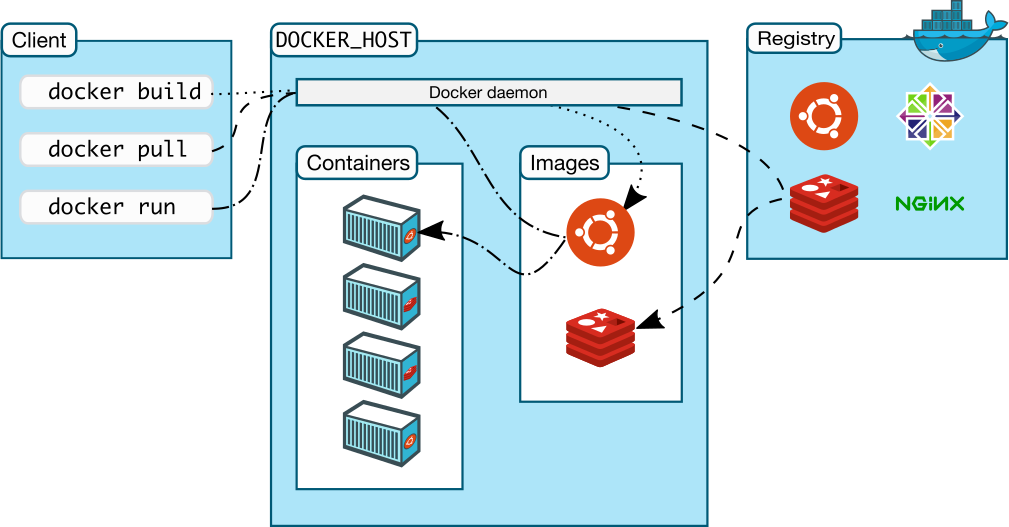
\includegraphics[width=0.75\linewidth]{figs/docker-architecture} 
\end{center}

The above figure is from the
\href{https://docs.docker.com/get-started/overview/}{official Docker overview} page.
\end{frame}

\begin{frame}[plain]{How Docker Works}
\framesubtitle{cont'd}
\begin{itemize}
\item
  Docker \textbf{images} are templates for creating a container. They
  are usually created from other images. For instance, an \emph{rstudio
  server image} would:
  \begin{enumerate}
  \item
    start from an Ubuntu image,
  \item
    update system libraries,
  \item
    install R and a base set of packages, and then finally
  \item
    install Rstudio.
  \end{enumerate}
\item
  If I wished to create an \emph{rstudio + jupyter server image}, I
  could build on top of the previous one, by adding instructions to:

  \begin{enumerate}
  \item
    install Python, and then
  \item
    install pip, jupyter and other required modules.
  \end{enumerate}
\item
  Instructions are stored in a textfile, known as a \texttt{Dockerfile}.
  Each line in a Dockerfile is cached as a layer so that it can re-used
  by other images.
\end{itemize}
\end{frame}

\begin{frame}{How Docker Works}
\framesubtitle{cont'd}

\begin{itemize}
\item
  Docker \textbf{containers} are runnable instances of images. Several
  containers from a single image can run on the same host.
\item
  We can create, start, stop containers based on images.
\item
  We can attach storage to them, so that containers can access files on
  our host machine. These are known as volumes.
\item
  We can even ``connect'' to containers and manipulate them as they are
  running. We can then commit the updated container to a new image and
  use it later.
\item
  Containers can communicate with one another.
\item
  Images can be stored online at a \textbf{registry}. One such registry
  is \href{https://hub.docker.com/}{docker hub}.
\end{itemize}
\end{frame}

\section{Introduction to Linux}
\frame{\tableofcontents[currentsection]}

\begin{frame}{Introduction to Linux}
\begin{columns}
\begin{column}{7.5cm}
\begin{itemize}
\item
  The Linux project was started in 1991 by Linus Torvalds.
\item
  UNIX had been used in servers everywhere since the 1960s.
\item
  Linux took the best things about UNIX (architecture, philosophy) and
  open-sourced it.
  \begin{itemize}
  \item
    \emph{Each program should do one thing, and do it well.}
  \end{itemize}
\end{itemize}
\end{column}
\onslide<2->
\begin{column}{7.5cm}
\begin{itemize}
\item
  Linux is
  \begin{itemize}
  \item
    free (as in speech),
  \item
    stable,
  \item
    fast,
  \item
    highly customisable, and is
  \item
    the best OS for coding in (personal opinion).
  \end{itemize}
\item
  Today Linux is run on many different platforms (small memory,
  in-memory, large, old hardware, high-end, budget):
  \begin{itemize}
  \item
    Android and ChromeOS are both based on Linux.
  \end{itemize}

\end{itemize}
\end{column}
\end{columns}
\vfill
\onslide<3->
  \emph{Did you know Mac OS is based on FreeBSD, which is a flavour of
  UNIX?}
\end{frame}


\begin{frame}{Linux Variants}
\begin{itemize}
\item
  There are many variants of Linux - they are fondly referred to as
  distributions or distros.
\item
  They all use the same Linux kernel, but come pre-packaged with
  different GUIs, and package management systems.
\item
  Take a look at this
  \href{https://upload.wikimedia.org/wikipedia/commons/b/b5/Linux_Distribution_Timeline_21_10_2021.svg}{stunning
  interactive visualisation} from wikipedia.
\item
  Intimidating as it appears, all distros have common elements that we
  can depend on.
\item
  The next figure is from
  \href{https://tldp.org/LDP/intro-linux/html/sect_03_01.html}{the Linux
  documentation project}.
\end{itemize}
\end{frame}

\begin{frame}[plain]{Directory Structure}
\begin{center}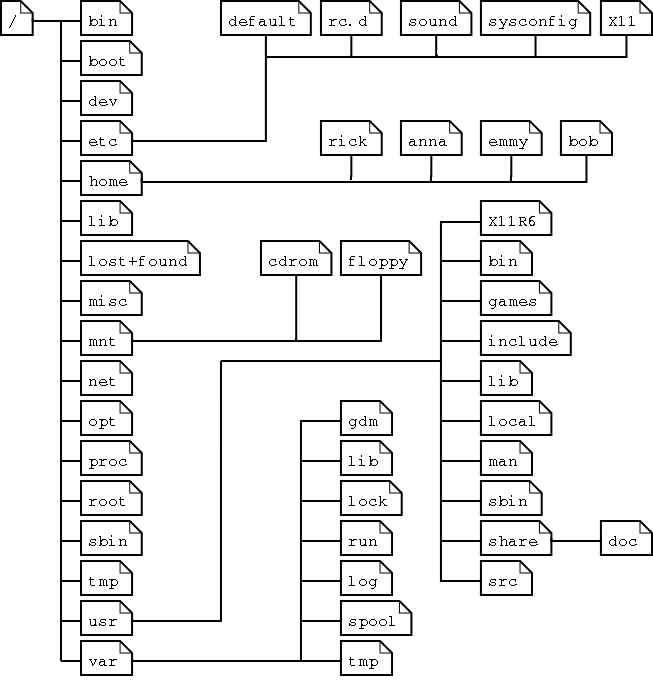
\includegraphics[width=0.5\linewidth]{figs/linux-filesystem-layout} 
\end{center}
\end{frame}

\begin{frame}{Directory Structure}
\renewcommand{\arraystretch}{1.1}
\begin{tabular}{ll}
\hline
Name & Content \\
\hline
/bin & Common programs, shared by the system, the system administrator
and the users. \\
/boot & The startup files and the kernel, vmlinuz. \\
/dev & Contains references to all the CPU peripheral hardware \\
/etc & Most important system configuration files are in /etc \\
/home & Home directories of the common users. \\
/lib & Library files, includes files for several programs needed by the
system and the users. \\
/lost+found & Files that were saved during failures are here. \\
/mnt & Standard mount point for external file systems, e.g.~a CD-ROM or
a digital camera. \\
/opt & Typically contains extra and third party software. \\
/root & The administrative user's home directory. \\
/sbin & Programs for use by the system and the system administrator. \\
/tmp & Temporary space for use by the system, cleaned upon reboot. \\
/usr & Programs, libraries, documentation etc. for all user-related
programs. \\
/var & Storage for all variable files and temporary files created by
users \\
\hline
\end{tabular}
\renewcommand{\arraystretch}{1}
\end{frame}

\begin{frame}{Installing Packages in Linux}
\begin{itemize}
\item
  To install packages on Linux machines, we need elevated privileges. We
  obtain this with the \texttt{sudo} command.
\item
  There are two main types of distributions, separated by their package
  types:
  \begin{itemize}
  \item
    RPM-based: examples are CentOS, Red Hat, Fedora. Use
    \texttt{sudo\ yum\ install\ xxx}
  \item
    Deb-based: examples are Debian, Ubuntu, Knoppix. Use
    \texttt{sudo\ apt\ install\ xxx}
  \end{itemize}
\item
  Docker images use Alpine linux because it is small. Use
  \texttt{apk\ install\ xxx} for Alpine-based images.
\end{itemize}

\end{frame}


\begin{frame}[fragile]{Installing Packages in Linux}
\framesubtitle{cont'd}
\begin{itemize}
\item
  We seldom have to do this any more.
\item
  The typical steps to install a package from source are:
\begin{lstlisting}
> tar -xvf xxx.tar.gz # unzip files
> cd xxx/           # Look around, read README, INSTALL files.
> ./configure       # Configures the installation script for our 
                    # machine.
                    # Take a toilet break!
                  
> make              # Compiles the code to create binaries and 
                    # shared libraries.
                    # At this point, the program can be run by 
                    # user.
                    # (Runs the Makefile.)
                    # Go have lunch and come back.
                  
> make install      # Requires sudo; installs binaries system-wide
                    # Stick around.
\end{lstlisting}

\end{itemize}
\end{frame}


\section{Writing Dockerfiles}
\frame{\tableofcontents[currentsection]}

\begin{frame}[fragile]{Dockerfiles}
\begin{itemize}
\item
  A Dockerfile is a text file that collects a set of instructions, to be
  run on the command line, in order to build a new image \textbf{from}
  an older image.
\item
  Once built, the containers can be run off that image.
\item
  A Dockerfile contains instructions of the form:

\begin{lstlisting}

# Comment
INSTRUCTION arguments

\end{lstlisting}
\item
  The first instruction must be \texttt{FROM}.
\item
  The important commands to be aware of are \texttt{RUN}, \texttt{CMD}
  and \texttt{ENTRYPOINT}.
\end{itemize}

\end{frame}

\begin{frame}[fragile]{Dockerfiles}
\begin{itemize}
\item
  \texttt{RUN} executes commands \textbf{only at build time}. There are
  two forms:

\begin{lstlisting}
# runs in a Bourne shell (i.e., /bin/sh not bash shell)
# The actual command is "/bin/sh -c echo $USER"
RUN echo $USER

# not run in any shell, so no variable expansion takes place
# (no output)
RUN ["echo", "$USER"]

# runs in a bash shell
RUN ["/bin/bash", "-c", "echo $USER"]

\end{lstlisting}
\item \texttt{CMD} has a similar set of variants, but it is run only when the 
image is run, \emph{not when it is built.}
\end{itemize}

\end{frame}

\begin{frame}[fragile]{Sample Dockerfile}
\begin{itemize}
\item Here is a sample Dockerfile, taken from 
\href{https://docs.docker.com/get-started/02_our_app/}{Docker help}.
\begin{lstlisting}
# syntax=docker/dockerfile:1
FROM node:12-alpine
RUN apk add --no-cache python2 g++ make
WORKDIR /app
COPY . .
RUN yarn install --production
CMD ["node", "src/index.js"]
EXPOSE 3000
\end{lstlisting}
\end{itemize}
\end{frame}

\begin{frame}{Volumes}
\begin{columns}
\begin{column}{7.5cm}
\begin{itemize}
\item
  As you observed in our \texttt{nginx} example, data in a container does not
  persist.
\item
  Once we remove a container, the data that was created inside it is
  lost.
\item
  To persist the data, we can use Docker volumes (preferred), or we can
  use bind mounts.
\item
  Bind mounts are managed by us; volumes are managed by Docker. In the 
  \texttt{nginx} example, we used a bind mount. 
\item Here is an example of using a volume to persist a database 
\href{https://docs.docker.com/get-started/05_persisting_data/}{across 
container restarts}.
\end{itemize}
\end{column}

\begin{column}{7.5cm}
\begin{center}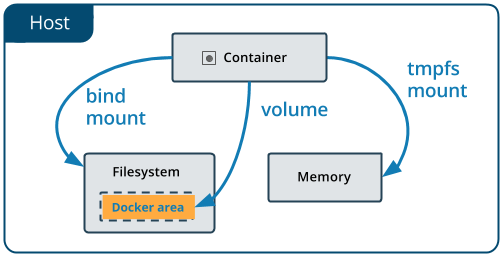
\includegraphics[width=0.75\linewidth]{figs/docker-types-of-mounts-volume} 
\end{center}
\end{column}

\end{columns}
\end{frame}

\section{Using Docker Compose}
\frame{\tableofcontents[currentsection]}

\begin{frame}{Getting Containers to Communicate}
\begin{itemize}
\item
  Containers are not meant to work in silos. In order to access a
  service on a container, we have to expose a port(s) to the host.
  \begin{itemize}
  \item
    There are 65536 possible ports (16-bit integer).
  \item
    This allows us to pretend that the container is a native
    application, listening on that port.
  \end{itemize}
\item
  Servers \emph{listen} on particular ports so that multiple services
  can run on a single host.
\item
  When a container is spun up, it is assigned an IP address, but this is
  on a private network.

  \begin{itemize}
  \item
    Special IP address: \texttt{127.0.0.1} and \texttt{localhost} refer
    to our host machine. We do not need the internet to reach this
    address.
  \end{itemize}
\end{itemize}
\end{frame}


\begin{frame}{Network Options}

\begin{enumerate}
\def\labelenumi{\arabic{enumi}.}
\item
  We can run containers with \texttt{-\/-network\ host}, which means
  that it the container is not isolated from the host.
    \begin{itemize}
    \item
      Only available on Linux hosts.
    \end{itemize}
\item
  We can define a Docker bridge network, and then assign containers to
  run on this network. We can then access containers by their name.
\item 
  Use docker compose to automatically create this network, start up all
  containers, and then add them to this network
    \begin{itemize}
    \item
      Containers are accessible by their names here, too.
    \end{itemize}

\end{enumerate}
\end{frame}


\section{Misc}
\frame{\tableofcontents[currentsection]}


\begin{frame}{Best Practices}
\begin{enumerate}
\def\labelenumi{\arabic{enumi}.}
\item
  Keep images small. If you just need Python, don't use \texttt{ubuntu},
  but \texttt{python} image.
\item
  Store data using volumes. This keeps containers isolated from the
  data, and easily replaceable.
\item
  Integrate your images with github actions to automatically push and
  test and tag images.
\end{enumerate}

\end{frame}


\begin{frame}{Container Orchestration}
\begin{itemize}
\item
  When deploying containers, an orchestration engine is used.
\item
  An example of this is Kubernetes.
\item
  This manages redundancies, allows for scaling up or down.
\item
  Learn more about Kubernetes
  \href{https://kubernetes.io/docs/tutorials/}{here}.
\end{itemize}
\end{frame}

\begin{frame}{Summary}
\begin{quote}
\emph{Sorry, why are we learning about Docker again?}
\end{quote}

\begin{itemize}
\item
  It will allow you to quickly code up a proof-of-concept to show how
  your model/product can be delivered.
\item
  With it, you can bravely use and connect up different services and
  applications in your product without fear of

  \begin{itemize}
  \item
    not being able to install it on your machine, and
  \item
    not being able to install it on others' (end-user, management, or
    production) machines.
  \end{itemize}
\item
  Knowing how containers can be deployed and scaled provides an
  appreciation of the machine engineering pipeline.
\end{itemize}

\end{frame}


\begin{frame}{References}
\begin{enumerate}
\def\labelenumi{\arabic{enumi}.}
\item
  \href{https://docs.docker.com/}{Docker Documentation}
\item
  \href{https://docs.docker.com/engine/reference/builder/}{Dockerfile
  Reference}
\item
  \href{https://go.exlibris.link/JCCDX7Gq}{Deploy Machine Learning
  Models to Production (book)}
\item
  \href{https://go.exlibris.link/SW8KgJVr}{Practical Docker with Python
  (book)}
\item
  \href{https://tldp.org/LDP/intro-linux/html/index.html}{Introduction
  to Linux}
\item
  \href{https://tldp.org/LDP/Bash-Beginners-Guide/html/index.html}{Bash
  Guide for Beginners}
\end{enumerate}

\end{frame}

%\begin{frame}{What is git?}
%\begin{columns}[T]
%\begin{column}{7.5cm}
%\begin{center}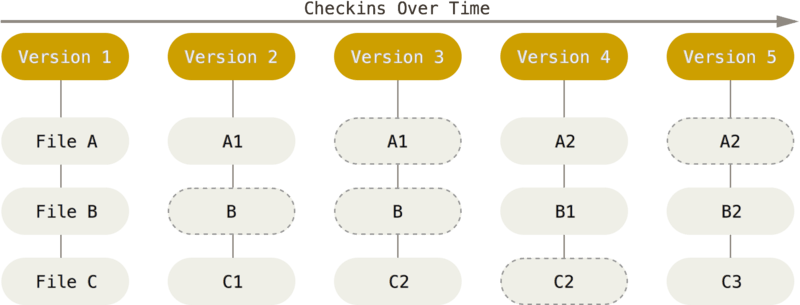
\includegraphics[width=0.8\linewidth]{figs/git-snapshots} \end{center}
%\end{column}
%\begin{column}{7.5cm}
%\begin{center}
%\begin{itemize}
%\item
%  git is a version control software.
%\item
%  With git, we do not need to worry about keeping track of multiple
%  versions of a file or a function.
%\item
%  We can test new features bravely, without worrying about how to get
%  back to an older, working version.
%\item
%  We can rollback to a previous/alternate version of the code at
%  anytime. Nothing is ever lost.
%\item
%  You can use git on your own, or you can use git as part of a team of
%  developers.
%\item
%  git is distributed.
%\item
%  \emph{git is not the same as github.} You can use git with or without
%  github.
%\end{itemize}
%\end{center}
%\end{column}
%\end{columns}
%\end{frame}
%
%
%\begin{frame}{Mental Model}
%\begin{columns}[T]
%\begin{column}{7.5cm}
%\begin{center}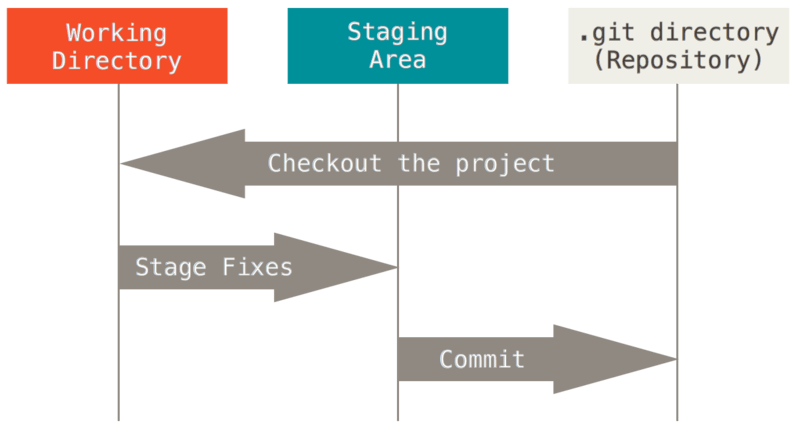
\includegraphics[width=0.85\linewidth]{figs/git-three-areas} 
%\end{center}
%\end{column}
%\begin{column}{7.5cm}
%\begin{itemize}
%\item
%  \emph{Working directory}: A single checkout of one version of the
%  project. Also referred to as \emph{working tree}.
%\item
%  \emph{Staging area}: A temporary, intermediate area that stores
%  information about your next commit (version that will be recorded and
%  stored). Changes from the working directory need to be
%  manually/consciously added to the staging area. The staging area is
%  also commonly referred to as the \emph{index}.
%\item
%  \emph{Repository}: A database of objects (files, meta information,
%  commit objects). Changes are not permanent until they have been
%  committed.
%\end{itemize}
%\end{column}
%\end{columns}
%\end{frame}
%
%\begin{frame}{Mental Model}
%\framesubtitle{cont'd}
%\begin{columns}[T]
%\begin{column}{7.5cm}
%\begin{center}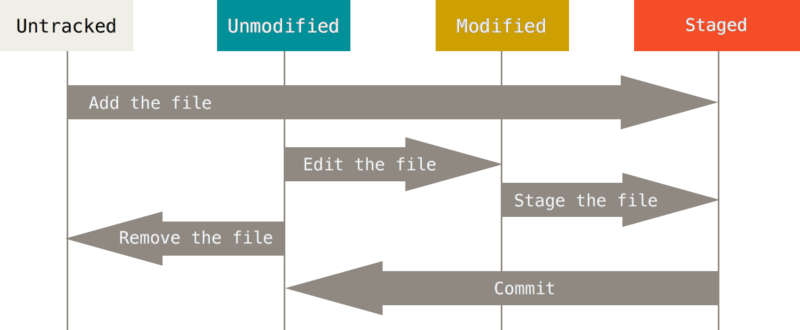
\includegraphics[width=0.8\linewidth]{figs/git-lifecycle} 
%\end{center}
%\end{column}
%\begin{column}{7.5cm}
%\begin{itemize}
%\item
%  A file in our working directory can be either \emph{tracked} or
%  \emph{untracked}. A tracked file is something git knows about; we can
%  stage and commit it.
%\item
%  Once tracked, a file is either
%  \begin{itemize}
%  \item
%    unmodified: the same as the file in the latest version of the
%    repository.
%  \item
%    modified: contains changes from the repository version, but not yet
%    staged.
%  \item
%    staged: ready to be committed.
%  \end{itemize}
%\item
%  git does not dictate how, or if, you use the staging area. You can
%  skip it altogether, every time, if you prefer to work that way.
%\end{itemize}
%\end{column}
%\end{columns}
%\end{frame}
%
%
%\begin{frame}{Terminology}
%\begin{columns}[T]
%\begin{column}{7.5cm}
%\begin{center}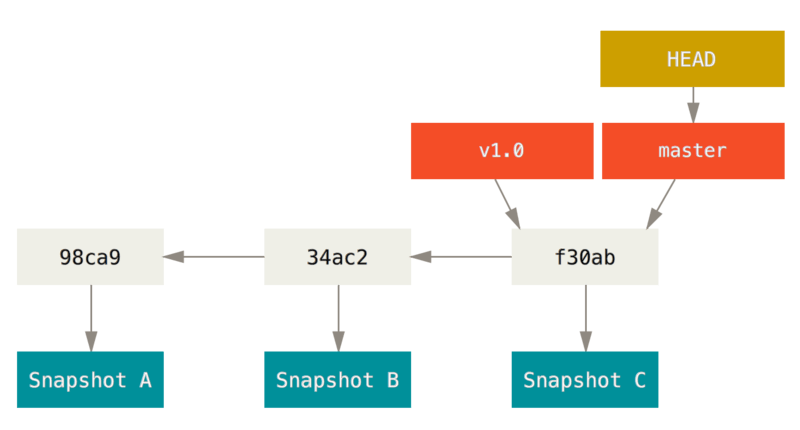
\includegraphics[width=0.75\linewidth]{figs/git-branch-and-history-01} 
%\end{center}
%\end{column}
%\begin{column}{7.5cm}
%\begin{itemize}
%\item
%  Each commit or snapshot is assigned a hash, using SHA-1. This is a
%  160-bit checksum.
%\item
%  In fact, in the object database, every file is named according to its
%  SHA-1 hash.
%\item
%  \texttt{98ca9} commit is the parent of \texttt{34ac2} commit in this
%  diagram.
%\item
%  There is only a single branch in this repository (master).
%\item
%  HEAD is a special pointer, that keeps track of which branch you are
%  currently on.
%\item
%  v1.0 is a tag; a friendly name for a commit.
%\end{itemize}
%\end{column}
%\end{columns}
%\end{frame}
%
%\begin{frame}[plain]{Example Workflow (Forward)}
%\begin{center}
%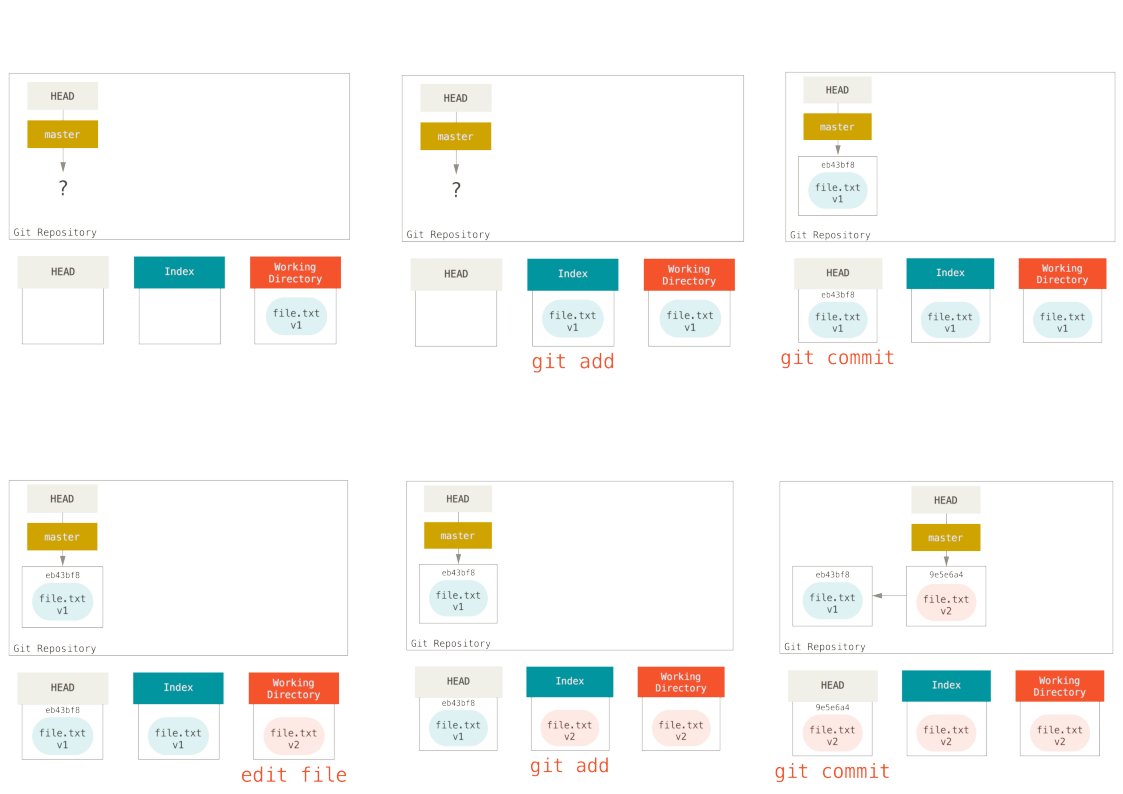
\includegraphics[width=0.7\linewidth]{figs/git_workflow_01} 
%\end{center}
%\end{frame}
%
%\begin{frame}[plain]{Example Workflow (Back)}
%\begin{center}
%\begin{center}\includegraphics[width=0.7\linewidth]{figs/git_reset_workflow} \end{center}
%\end{center}
%\end{frame}
%
%\begin{frame}{Git Branching}
%\begin{center}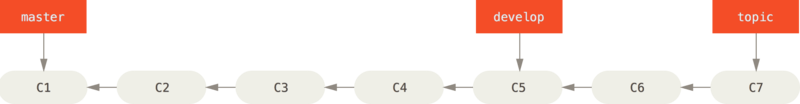
\includegraphics[width=0.6\linewidth]{figs/git-lr-branches-1} \end{center}
%
%\begin{center}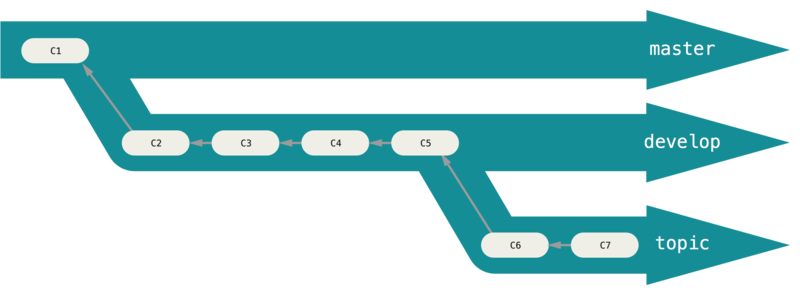
\includegraphics[width=0.6\linewidth]{figs/git-lr-branches-2} \end{center}
%\end{frame}
%
%
%\begin{frame}{Git Branching}
%\framesubtitle{cont'd}
%\begin{itemize}
%\item
%  To test out new features/debug things, we can create new branches.
%\item
%  In git, this is fast and lightweight.
%\item
%  There are three branches here: \texttt{develop} is ahead of
%  \texttt{master}, and \texttt{topic} is further ahead of
%  \texttt{develop}.
%\item
%  We can work on experimental new features in \texttt{develop}, while
%  the main codebase in \texttt{master} remains stable in production.
%\end{itemize}
%\end{frame}
%
%\begin{frame}[plain]{Local Branches}
%\begin{center}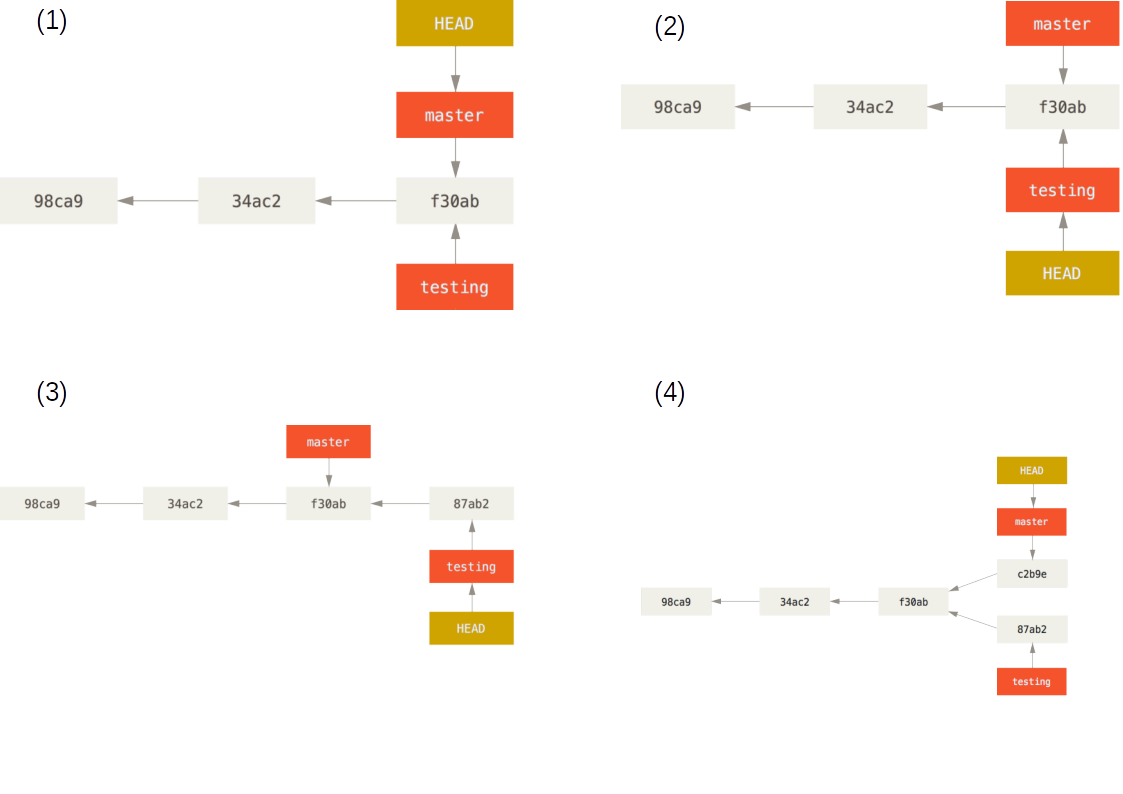
\includegraphics[width=0.75\linewidth]{figs/branching_seq_01} \end{center}
%\end{frame}
%
%\begin{frame}[plain]{Remote Branches}
%\begin{center}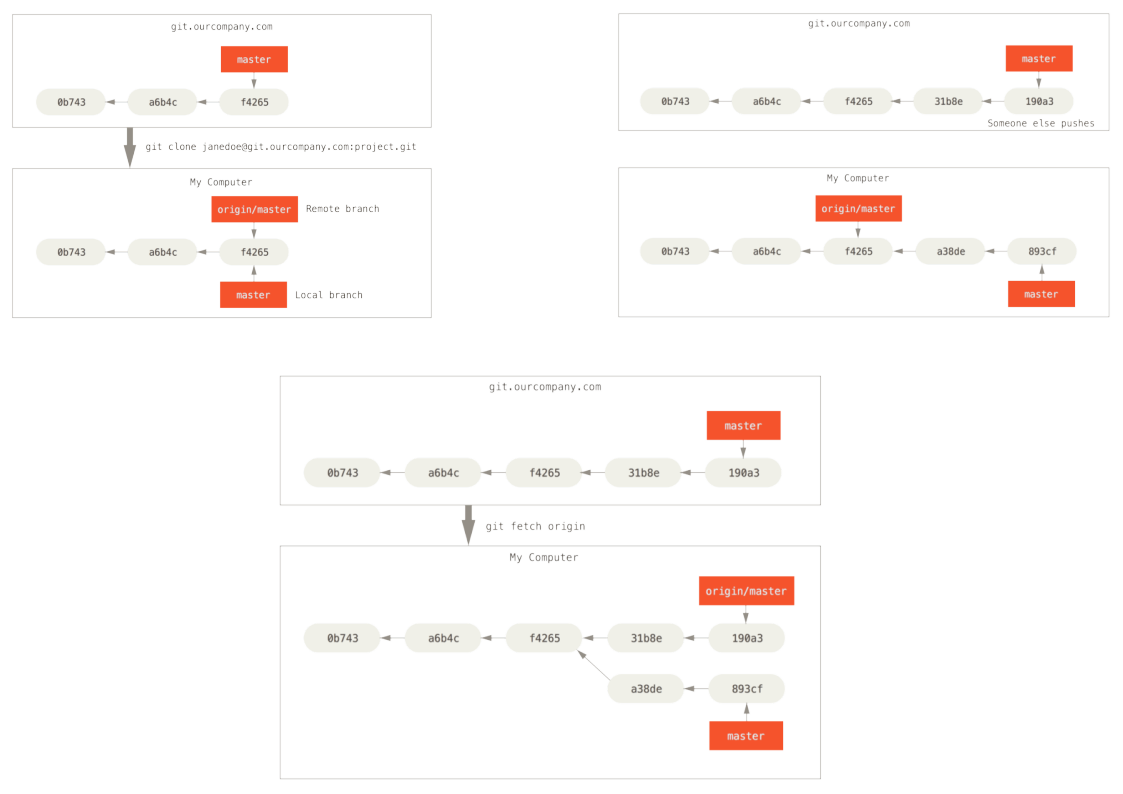
\includegraphics[width=0.75\linewidth]{figs/branching_seq_02} 
%\end{center}
%\end{frame}
%
%\begin{frame}[plain]{Integrating Changes}
%\begin{center}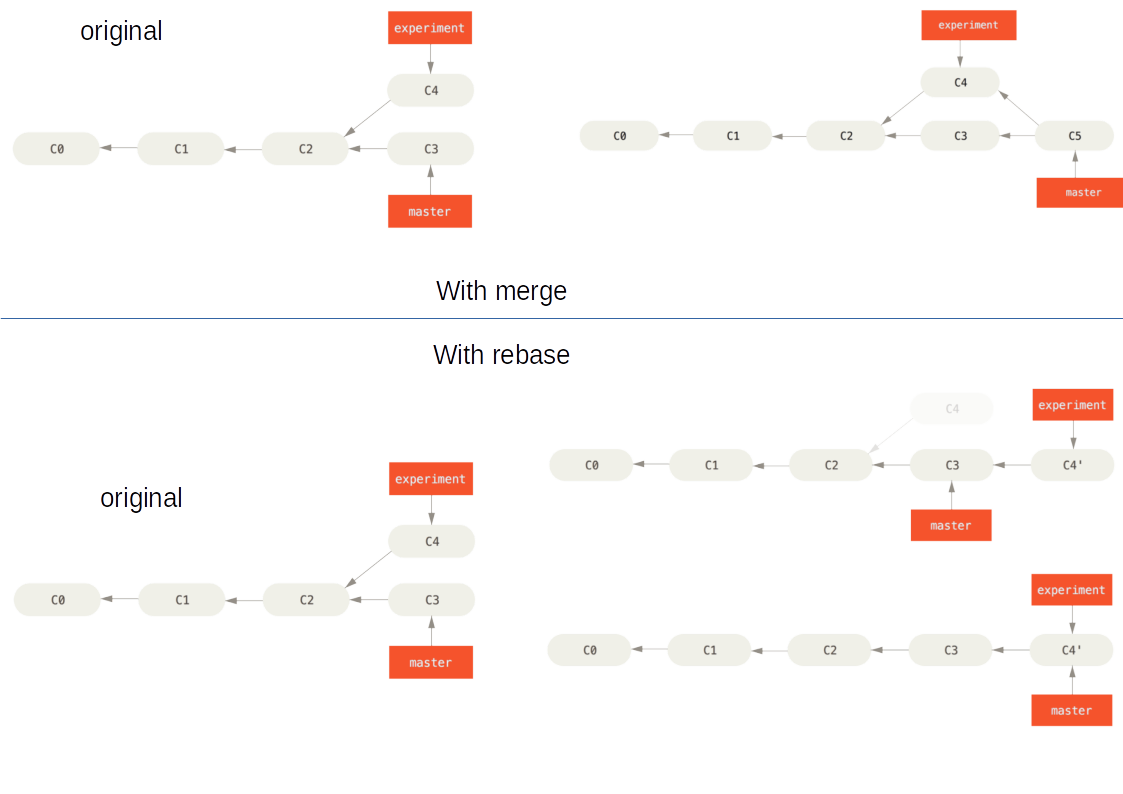
\includegraphics[width=0.75\linewidth]{figs/rebase_example} 
%\end{center}
%\end{frame}
%
%\begin{frame}{Ignoring Files}
%\begin{itemize}
%\item
%  The \texttt{.gitignore} file contains patterns that let git know which
%  files should intentionally not be tracked.
%\item
%  A separator \texttt{/} at the end of a line indicates that it is a
%  folder that should be ignored.
%\end{itemize}
%\begin{block}{Examples}
%\begin{enumerate}
%\def\labelenumi{\arabic{enumi}.}
%\item
%  \texttt{hello.*} matches any file or directory that begins with
%  \texttt{hello.}
%\item
%  \texttt{/hello.*} matches \texttt{hello.R} but not
%  \texttt{dir1/hello.R} (pattern restricted to only this directory).
%\item
%  \texttt{foo/} will match a directory and everything under it, but not
%  any file named \texttt{foo}.
%\item
%  \texttt{foo/*} will match any files under the directory \texttt{foo},
%  but not \texttt{foo/bar/hello.R}. The asterisk does not match the
%  \texttt{/} separator character.
%\end{enumerate}
%\end{block}
%\end{frame}
%
%\begin{frame}{Common Commands}
%\begin{itemize}
%\item
%  \texttt{git\ add} (interactive option available), \texttt{git\ commit}
%\item
%  \texttt{git\ diff}, \texttt{git\ log}, \texttt{git\ show},
%  \texttt{git\ blame}
%\item
%  \texttt{git\ checkout}, \texttt{git\ switch}, \texttt{git\ branch}
%\item
%  \texttt{git\ reset}, \texttt{git\ restore}
%\item
%  \texttt{git\ push}, \texttt{git\ pull}, \texttt{git\ fetch},
%  \texttt{git\ remote}
%\item
%  \texttt{git\ merge}, \texttt{git\ rebase}
%\end{itemize}
%\end{frame}
%
%\begin{frame}{Using Staging}
%\begin{enumerate}
%\def\labelenumi{\arabic{enumi}.}
%\item
%  When working, I frequently make small changes and test them. Each time
%  a small change is working, I stage it so that my working tree is
%  clean. Now \texttt{git\ diff} will only highlight the next small
%  change I am working on.
%\item
%  Sometimes, I have made many changes to many files without committing
%  or staging. Committing them at one go would not be meaningful. With
%  the staging area, I can stage and commit the changes (even partial
%  file changes) one group at a time.
%\item
%  If you do not feel this is how you would like to work, feel free to
%  use
%
%\begin{itemize}
%\item
%  \texttt{git\ status\ -s}
%\item
%  \texttt{git\ commit\ -a} 
%\item The latter command will automatically stage
%  and then commit the modified files in your working tree. \emph{This
%  skips the staging area.}
%\end{itemize}
%\end{enumerate}
%
%\end{frame}
%
%
%\begin{frame}{git Command Line}
%\begin{itemize}
%\item
%  The git command line works from the git-bash shell.
%  \begin{itemize}
%  \item
%    Full documentation for every command is accessible through
%    \texttt{git\ \textless{}command\_name\textgreater{}\ -\/-help}.
%  \end{itemize}
%\item
%  Several commands can take revisions, and file paths as input.
%  \begin{itemize}
%  \item
%    A revision can be a commit, branch or a tag
%  \end{itemize}
%\item
%  Revisions and file paths can be separated using \texttt{-\/-}
%\end{itemize}
%
%\begin{block}{Examples}
%\begin{itemize}
%\item
%  \texttt{git\ show\ abde09}
%  \begin{itemize}
%  \item
%    Provides details about commit that begins with abde09.
%  \end{itemize}
%\item
%  \texttt{git\ show\ abde09\ -\/-\ test.sql}
%  \begin{itemize}
%  \item
%    Provides details about file test.sql in commit that begins with
%    abde09.
%  \end{itemize}
%\item
%  \texttt{git\ diff\ 6c05cfc..b1ab8f7\ \ -\/-\ src/01\_git\_workshop.Rmd}
%  \begin{itemize}
%  \item
%    Shows differences between file \texttt{src/01\_git\_workshop.Rmd}
%    between older commit \texttt{6c05cfc} and newer commit
%    \texttt{b1ab8f7}.
%  \end{itemize}
%\end{itemize}
%\end{block}
%\end{frame}
%
%
%\begin{frame}[plain]{Common Distributed Workflows}
%\begin{center}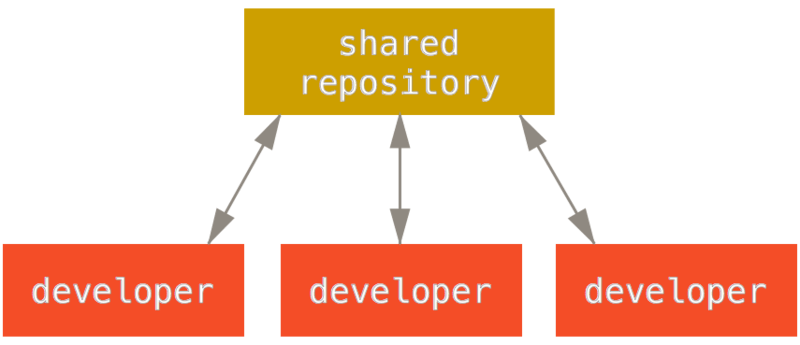
\includegraphics[width=0.75\linewidth]{figs/centralized_workflow} 
%\end{center}
%\end{frame}
%
%\begin{frame}[plain]{Common Distributed Workflows}
%\framesubtitle{cont'd}
%\begin{center}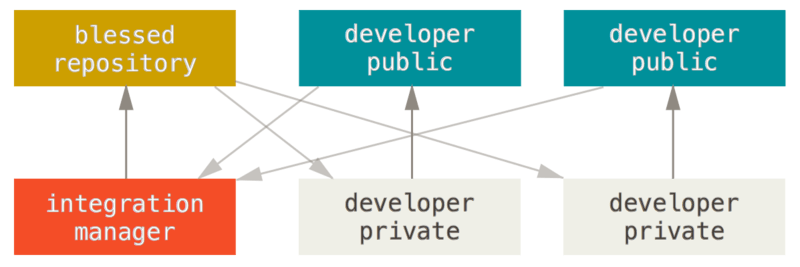
\includegraphics[width=0.75\linewidth]{figs/integration-manager} 
%\end{center}
%\end{frame}
%
%
%\begin{frame}{Good Advice}
%\begin{columns}
%\begin{column}{7.5cm}
%\begin{enumerate}
%\def\labelenumi{\arabic{enumi}.}
%\item
%  The \href{https://www.git-scm.com/}{git website}.
%\item
%  A very neat
%  \href{https://ndpsoftware.com/git-cheatsheet.html}{interactive
%  visualisation}
%\item
%  On \href{http://www-cs-students.stanford.edu/~blynn/gitmagic/}{the
%  magic of git}.
%\item
%  Github \href{https://docs.github.com/en}{documentation pages}.
%\end{enumerate}
%\end{column}
%\onslide<2>
%\begin{column}{7.5cm}
%\begin{enumerate}
%\def\labelenumi{\arabic{enumi}.}
%\item
%  Use it for your own single-person projects.
%\item
%  Use it in school projects.
%\end{enumerate}
%
%Do not be afraid of ``breaking'' things. With git, it is almost
%\emph{always} possible to recover.
%
%\end{column}
%\end{columns}
%\end{frame}

\end{document}
